% typ dokumentu
\documentclass[12pt,twoside]{article}

% użycie pakietu , jak include
\usepackage{weiiszablon}

% autor pracy
\author{Krystian Olszowy}

% np. EF-123456, EN-654321, ..., Numer albumu
\studentID{EA-167582}

\title{Tworzenie drzewa składniowego języka ST}
\titleEN{{Creating an ST language syntax tree}}


%%% wybierz rodzaj pracy wpisując jeden z poniższych numerów: ...
% 1 = inżynierska	% BSc
% 2 = magisterska	% MSc
% 3 = doktorska		% PhD
%%% na miejsce zera w linijce poniżej
\newcommand{\rodzajPracyNo}{2}


%%% promotor
\supervisor{dr inż. Jan Sadolewski}
%% przykład: dr hab. inż. Józef Nowak, prof. PRz

%%% promotor ze stopniami naukowymi po angielsku
\supervisorEN{Jan Sadolewski, PhD, Eng.}


%% DO ZROBIENIA %%
\abstract{Praca zawiera zaproponowane rozwiązanie sterowania telewizorem z poziomu smartfona dzięki aplikacji mobilnej i urządzeniu pośredniczącemu, opartemu o mikrokontroler z niezbędnymi modułami. Przedstawiono i omówiono w niej technologie i koncepty, z których korzystano podczas procesu projektowania i tworzenia rozwiązania. Opisane zostały też najważniejsze elementy fizycznej części systemu, oprogramowanie mikrokontrolera, zbudowana aplikacja mobilna oraz ich współpraca w celu sterowania urządzeniem telewizyjnym.}
\abstractEN{The work encompasses a solution for television control through a smartphone application and an intermediary device, based on a microcontroller with necessary modules. It introduces and discusses the technologies and concepts employed during the design and building process. Additionally, it details the key components of the physical system, microcontroller software, the developed mobile application, and their collaboration for television device control.}

%% DO ZROBIENIA %%
\keywords{ST language, syntax tree, CPDev, Flutter, aplikacja mobilna}
\keywordsEN{remote controller, BLE, IR, Flutter, mobile application}


\begin{document}

% strona tytułowa
\maketitle

\blankpage

% spis treści
\tableofcontents

\clearpage
\blankpage

\section{Wstęp}
\subsection{Zintegrowane środowiska programistyczne (ang. IDE)}
Współczesny inżynier czy programista automatyki nie wyobraża sobie pracy bez dostępu do zintegrowanego środowiska programistycznego (ang. IDE). Środowiska te, będące podstawowym narzędziem w pracy twórców oprogramowania sterowników PLC, przekształciły się z prostych edytorów kodu w zaawansowane platformy wspierające projektowanie, symulację, testowanie i wdrażanie systemów sterowania. Dzięki nim możliwe jest nie tylko wygodne tworzenie logiki sterującej, ale również wizualizacja procesów, zarządzanie konfiguracją sprzętu czy analizowanie działania programu w~czasie rzeczywistym.

Na rynku dostępnych jest wiele rozwiązań, różniących się zakresem funkcji, kompatybilnością z określonymi typami sterowników oraz poziomem zaawansowania użytkownika. Jednym z przykładów takiego środowiska jest CPDev - polskie oprogramowanie tworzone na Politechnice Rzeszowskiej wspierające języki programowania zgodne z normą IEC 61131-3, które umożliwia programowanie sterowników różnych producentów, symulację działania programu oraz jego późniejsze wdrożenie na urządzeniu docelowym. Choć wiele firm korzysta z komercyjnych środowisk oferowanych przez producentów sterowników, takich jak TIA Portal firmy Siemens czy GX Works rozwijane przez Mitsubishi Electronic, to rosnąca popularność rozwiązań niezależnych - jak CPDev - pokazuje, że możliwe jest tworzenie otwartych, elastycznych i konkurencyjnych narzędzi dla branży automatyki.

\subsection{Drzewa składniowe}
Drzewa składniowe to struktury, które trudno przecenić w świecie programowania. Choć na pierwszy rzut oka mogą wydawać się technicznym detalem, w~praktyce są fundamentem działania wielu elementów środowisk programistycznych. To właśnie one przedstawiają kod w uporządkowanej postaci, zgodnej z gramatyką danego języka, dzięki czemu program może być łatwiej analizowany i przetwarzany.

Bez drzew składniowych trudno wyobrazić sobie działanie kompilatorów, interpreterów, a nawet tak podstawowych funkcji edytora jak kolorowanie składni, podpowiadanie składniowe czy automatyczne formatowanie kodu. Dzisiejsze IDE bazują na tych strukturach niemal na każdym kroku - to one pozwalają na bieżąco wykrywać błędy kodu, usprawniają nawigację w projekcie i umożliwiają wprowadzenie inteligentnych podpowiedzi.

Automatyczne generowanie parserów, znacząco przyspiesza proces interpretacji kodu. Dzięki niemu programista nie musi już ręcznie tworzyć złożonych analizatorów składni, co oszczędza czas i~ogranicza liczbę błędów.

Dla środowiska CPDev możliwość generowania drzewa składniowego dla języka ST to istotne ułatwienie. Dzięki temu można nie tylko szybciej i prościej zaimplementować parser zgodny z normą IEC 61131-3, ale też stworzyć solidną podstawę do rozwijania edytora o nowe funkcje - jak choćby inteligentne podpowiedzi, analiza semantyczna czy lepsza diagnostyka błędów. To wszystko przekłada się na wygodniejszą pracę użytkownika i otwiera drogę do dalszego rozwoju CPDeva jako nowoczesnego narzędzia do programowania sterowników.

\subsection{Cel pracy}
Celem pracy jest przygotowanie parsera kodu języka ST zgodnego z normą IEC 61131-3 oraz oprogramowaniem CPDev, generującego drzewo składniowe na~podstawie podanego kodu źródłowego tego języka. Oprogramowanie generujące drzewo składniowe ma współpracować z kodem w języku C\#. Aby takie oprogramowanie przygotować, należy wcześniej także przeprowadzić badanie porównawcze wybranych narzędzi do tworzenia drzew składni języków formalnych opisanych za pomocą gramatyki bezkontekstowej i wybrać rozwiązanie najbardziej odpowiadające postawionemu zadaniu.

\subsection{Zakres pracy}
Zakres pracy obejmuje prównanie wybranych narzędzi do tworzenia drzew skła\-dni języków formalnych opisanych za pomocą gramatyki bezkontekstowej i wybranie najlepszego z nich do analizowania języka ST zgodnego z normą IEC 61131-3 w~CPDevie. Praca podejmuje także tematykę utworzenia pliku gramatyki języka ST dla najbardziej odpowiedniego z analizowanych narzędzi i przetestowania wygenerowanego oprogramowania dla przykładowych kodów źródłowych.


\subsection{Zawartość pracy [DO ZROBIENIA]}
W rozdziale drugim  omówiono ogólnodostępne rozwiązania stanowiące aktualny stan wiedzy w zakresie zdalnego sterowania odbiornikiem telewizyjnym. Prównano je z autorskim systemem wskazując jego zalety i rozwiązywane przez niego problemy.

Rozdział trzeci zawiera przedstawienie i opis technologii wykorzystanych w zaprojektowanym rozwiązaniu. Są to: Platforma ESP32, język programowania C++, framework Arduino, podczerwień, system Android, język programowania Dart, framework Flutter oraz techonlogia Bluetooth Low Energy.

Czwarty rozdział opisuje sposób połączenia komponentów składających się na urządzenie pośredniczące zbudowane aby skomunikować aplikację mobilną z telewizorem. Zawarte zostały w nim także opisane scharakteryzowane parametry tych komponentów.

W rozdziale piątym szczegółowo omówiono utworzone oprogramowanie mikrokontrolera odpowiedzialne za sterowanie jego zasobami i dołączonymi modułami fizyczymi. Przedstawione zostały ważniejsze kody źródłowe projektu oraz ich działanie.

Rozdział szósty zawiera opis zaprojektowanego intefejsu użytkownika aplikacji mobilnej oraz jej funkcjonalności. Ukazane zostały także wykorzystane podczas implementacji, rozwiązania programowe.

Siódmy rozdział koncentruje się na przedstawieniu sposobu korzystania z utworzonego rozwiązania. Dokonywana jest także ocena skuteczności działania poszczególnych funkcji systemu.

W ostatnim rozdziale zawarto podsumowanie całej pracy, możliwe usprawnienia zaprojektowanego rozwiązania. Wskazane zostały też elementy projektu, które autor uważa za wkład własny.


\clearpage
\section{Środowisko CPDev}
\subsection{Charakterystyka narzędzia}
CPDev (Control Program Developer) to otwarte, uniwersalne środowisko inżynierskie przeznaczone do tworzenia i wdrażania oprogramowania sterującego dla systemów automatyki. Powstało jako efekt wieloletnich prac badawczych i rozwojowych prowadzonych na Politechnice Rzeszowskiej. Głównym założeniem projektowym CPDev było stworzenie platformy, która będzie nie tylko zgodna z normą IEC 61131-3, ale również łatwa do przeniesienia na różne platformy sprzętowe i dostępna dla inżynierów oraz studentów jako narzędzie zarówno edukacyjne, jak i przemysłowe\cite{cpdevKia}.

Jednym z głównych atutów CPDev jest modularność oraz szeroki zakres funkcjonalności obejmujący cały proces tworzenia aplikacji sterujących. Środowisko udostępnia zestaw edytorów tekstowych i graficznych, narzędzia do konfiguracji systemu, symulator sterownika oraz narzędzia do projektowania interfejsów HMI. Dzięki temu możliwe jest kompleksowe projektowanie i testowanie systemów sterowania bez konieczności stosowania zewnętrznych narzędzi.

Ważną cechą CPDev jest jego niezależność sprzętowa, osiągnięta dzięki zastosowaniu warstwy pośredniej w postaci wirtualnej maszyny, która interpretuje kod pośredni generowany przez kompilator. Takie podejście umożliwia łatwe wdrażanie systemu na różnych urządzeniach, w tym na mikrokontrolerach, procesorach ARM, a nawet na implementacjach FPGA\cite{cpdevFPGA}. Jednocześnie zapewnia ono jednolity sposób działania aplikacji niezależnie od platformy sprzętowej.

Środowisko CPDev jest stale rozwijane i udoskonalane. W kolejnych wersjach wprowadzano m.in. wsparcie dla języków graficznych, rozszerzenia dla systemów wielordzeniowych, interfejsy XML pozwalające na współpracę z innymi narzędziami inżynierskimi oraz rozwiązania umożliwiające projektowanie zgodnie z podejściem MDD (Model-Driven Development). CPDev znalazł już zastosowanie w wielu wdrożeniach przemysłowych — zarówno w kraju, jak i za granicą.

Z punktu widzenia użytkownika, środowisko CPDev oferuje funkcjonalności znane z komercyjnych rozwiązań, przy czym wyróżnia się większą otwartością, możliwością adaptacji do konkretnych potrzeb oraz dostępnością szczegółów implementacyjnych. To wszystko sprawia, że CPDev stanowi atrakcyjną alternatywę wobec zamkniętych środowisk oferowanych przez producentów sprzętu automatyki.
\subsection{Programowanie za pomocą CPDev-a}
\subsubsection{Ogólny sposób korzystania z narzędzia}
Programowanie w środowisku CPDev odbywa się w ramach graficznego interfejsu IDE, które integruje różne etapy projektowania systemu automatyki: od pisania kodu sterującego, przez konfigurację sprzętu i symulację, aż po wdrożenie na urządzenie docelowe \cite{cpdev2009}. Proces ten można podzielić na kilka etapów:

\begin{enumerate}[label=\arabic*), leftmargin=1.25cm]
    \item Tworzenie projektu - użytkownik definiuje strukturę programu, dodaje nowe jednostki organizacyjne (POUs), deklaruje zmienne globalne i lokalne.
    \item Kodowanie logiki sterowania -- za pomocą jednego lub kilku języków normy IEC 61131-3.
    \item Konfigurację sprzętu i zmiennych wejścia-wyjścia -- z użyciem narzędzia CPCon.
    \item Symulację i testowanie -- możliwą dzięki narzędziu CPSim, które pozwala uruchomić aplikację sterującą w trybie offline.
    \item Generowanie kodu pośredniego (VMASM) -- po kompilacji, aplikacja może zostać załadowana do wirtualnej maszyny uruchamianej na docelowym sterowniku.
\end{enumerate}

\subsubsection{Dostępne języki programowania sterowników}
CPDev wspiera wszystkie języki określone w normie IEC 61131-3\cite{iec61131-3}, co pozwala użytkownikom wybrać najbardziej pasujący im sposób definiowania logiki sterującej w zależności od specyfiki projektu lub preferencji osobistych. Szczegółowo, obsługiwane przez CPDev języki programowania  to\cite{cpdevLanguages}:

\begin{enumerate}[label=\alph*), leftmargin=1.25cm]
    \item ST (Structured Text)\\
    Język ST jest tekstowym językiem wysokiego poziomu, przypominającym składnią Pascala lub języki z rodziny C. Oferuje bogaty zestaw struktur sterujących (pętle, warunki, bloki), obsługę typów prostych i złożonych oraz wyrażeń logicznych i arytmetycznych. CPDev umożliwia pisanie całych aplikacji w ST, a także używanie go do definiowania funkcji i bloków funkcyjnych. Edytor kodu ST w CPDev jest wyposażone w podświetlanie składni, autouzupełnianie i sprawdzanie błędów składniowych na bieżąco, co znacznie ułatwia pracę programisty. Okno edycji z przykładowym kodem ST przedstawiono na rysunku \ref{Fig:startStopST}.

   \begin{figure}[ht]
   \centering
   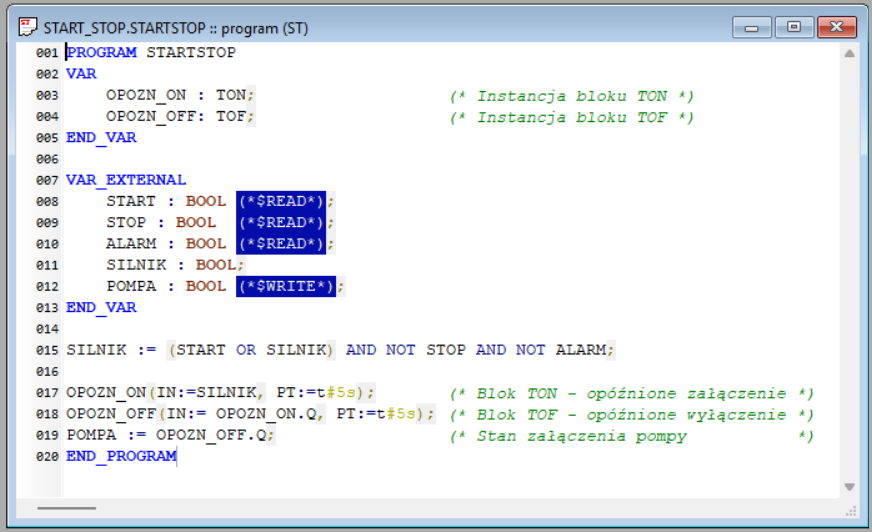
\includegraphics[width=12cm]{images/startStopST.png}
   \caption{Wygląd okna edycji prostego kodu ST w programie CPDev}
   \label{Fig:startStopST}
   \end{figure}

    \item IL (Instruction List)\\
    IL to język niskopoziomowy, przypominający asembler. Umożliwia precyzyjne określanie instrukcji operujących na rejestrach i zmiennych. Jego stosowanie w CPDev jest obecnie rzadsze, ponieważ został wycofany z najnowszej wersji normy IEC 61131-3, ale nadal pozostaje dostępny dla kompatybilności. Okno edycji IL w CPDev pozwala na pisanie kodu w formie instrukcji, przedstwiono je wraz z przykładowym kodem na rysunku \ref{Fig:startStopIL}. 

   \begin{figure}[ht]
   \centering
   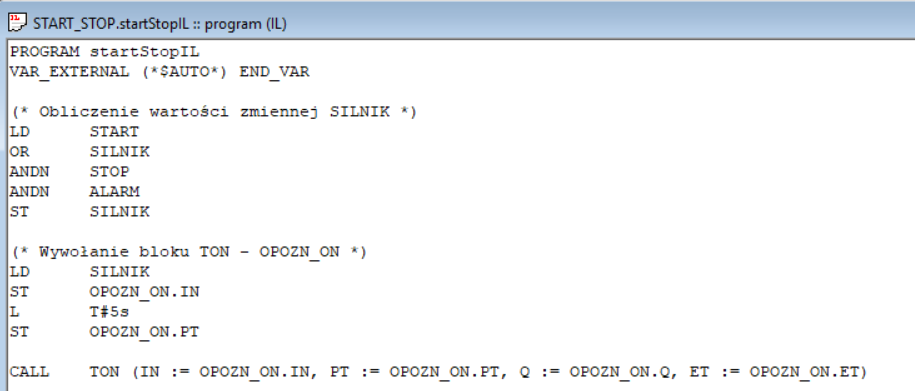
\includegraphics[width=13cm]{images/startStopIL.png}
   \caption{Wygląd okna edycji prostego kodu IL w programie CPDev}
   \label{Fig:startStopIL}
   \end{figure}

    \item FBD (Function Block Diagram)\\
    FBD jest językiem graficznym, który pozwala na tworzenie logiki poprzez łączenie bloków funkcyjnych w sposób przypominający schematy blokowe. Jest chętnie wykorzystywany przez inżynierów o mniejszym doświadczeniu programistycznym, szczególnie w przemyśle. W CPDev edytor FBD umożliwia tworzenie diagramów blokowych, gdzie każdy blok reprezentuje funkcję lub operację, a połączenia między nimi definiują przepływ danych. Bloki mogą być konfigurowane i łączone w sposób graficzny, co ułatwia zrozumienie logiki sterowania. Przykładowe okno edycji FBD z prostym kodem przedstawiono na rysunku \ref{Fig:startStopFBD}.

   \begin{figure}[ht]
   \centering
   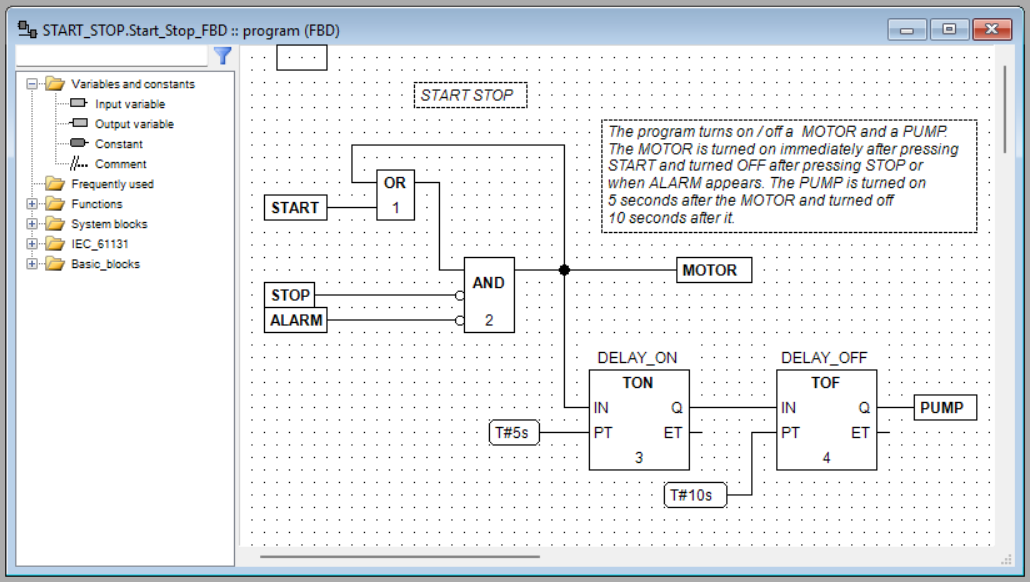
\includegraphics[width=14cm]{images/startStopFBD.png}
   \caption{Wygląd okna edycji prostego kodu FBD w programie CPDev}
   \label{Fig:startStopFBD}
   \end{figure}

    \item LD (Ladder Diagram)\\
    LD, znany także jako język drabinkowy, to język graficzny inspirowany schematami przekaźnikowymi. Ułatwia migrację klasycznych systemów sterowania przekaźnikowego do programowalnych sterowników PLC. CPDev umożliwia tworzenie programów w LD i konwersję do ST. Edytor LD pozwala na graficzne definiowanie logiki sterującej w formie drabinki, gdzie symbole reprezentują elementy logiczne (przekaźniki, styki, cewki), a połączenia między nimi definiują przepływ sygnałów. Przykładowe okno edycji LD z prostym kodem przedstawiono na rysunku \ref{Fig:startStopLD}.

   \begin{figure}[ht]
   \centering
   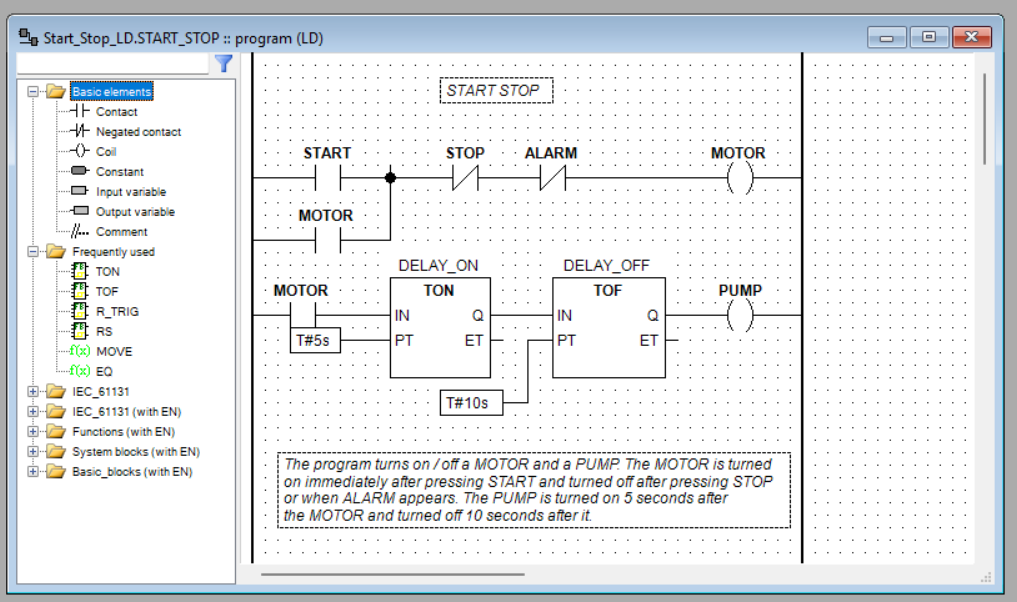
\includegraphics[width=12cm]{images/startStopLD.png}
   \caption{Wygląd okna edycji prostego kodu LD w programie CPDev}
   \label{Fig:startStopLD}
   \end{figure}

    \item SFC (Sequential Function Chart)\\
    SFC jest językiem służącym do modelowania logiki sekwencyjnej. Program składa się z kroków, przejść i warunków przejścia. W CPDev sekwencyjna struktura tworzona jest graficznie, a logika kroków i przejść może być zapisana w ST lub FBD. Edytor SFC w CPDev pozwala na tworzenie diagramów sekwencyjnych, gdzie każdy krok reprezentuje stan systemu, a przejścia między nimi definiują warunki przejścia. Przykładowe okno edycji SFC z prostym kodem przedstawiono na rysunku \ref{Fig:tanksSFC}.

   \begin{figure}[ht]
   \centering
   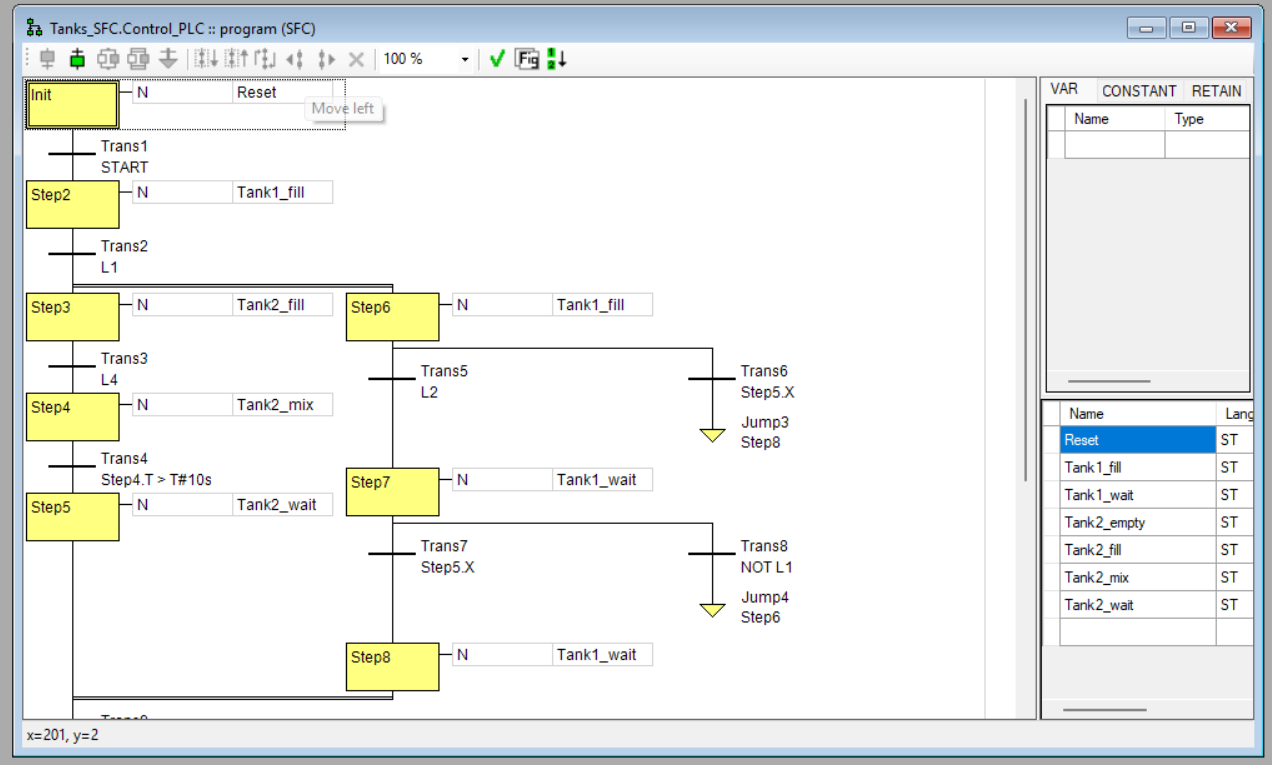
\includegraphics[width=12cm]{images/tanksSFC.png}
   \caption{Wygląd okna edycji prostego kodu SFC w programie CPDev}
   \label{Fig:tanksSFC}
   \end{figure}
\end{enumerate}

\subsection{Implementacja CPDev-a i architektura maszyny wirtualnej}

Implementacja środowiska CPDev została oparta na założeniu, że system sterowania powinien być niezależny od konkretnej platformy sprzętowej, a zarazem możliwy do wdrożenia w rzeczywistych aplikacjach przemysłowych. Aby to osiągnąć, architektura CPDev została podzielona na dwa główne poziomy: środowisko deweloperskie (IDE) oraz maszynę wirtualną (VM), która wykonuje wygenerowany program sterujący.

Środowisko deweloperskie CPDev zostało zaimplementowane w języku C\# na platformę .NET, przez co aplikacja posiada nowoczesny interfejs graficzny, wygodę użytkowania i łatwość dalszej rozbudowy. Składa się z modularnych komponentów, takich jak edytory kodu źródłowego, narzędzia konfiguracyjne, symulatory, analizatory błędów i generator kodu pośredniego \cite{cpdevOverview}. Zastosowanie C\# i środowiska .NET pozwala na integrację z innymi narzędziami, obsługę graficznych języków programowania oraz wprowadzanie rozwiązań typowych dla nowoczesnych aplikacji okienkowych (GUI).

Kluczowym elementem działania środowiska jest kompilator, który tłumaczy kod źródłowy napisany w językach normy IEC 61131-3 (głównie ST) do VMASM - pośredniego kodu niskiego poziomu wykonywanego przez maszynę wirtualną. Maszyna wirtualna CPDev-a to lekki, niezależny od sprzętu interpreter kodu VMASM, implementowany głównie w języku ANSI C, co zapewnia wysoką przenośność. Dzięki temu może ona działać na wielu różnych platformach sprzętowych, w tym na mikrokontrolerach (np. AVR, ARM), systemach wbudowanych (np. Raspberry Pi, STM32), a także w symulacji na komputerze PC\cite{cpdevVM}.

\begin{figure}[ht]
   \centering
   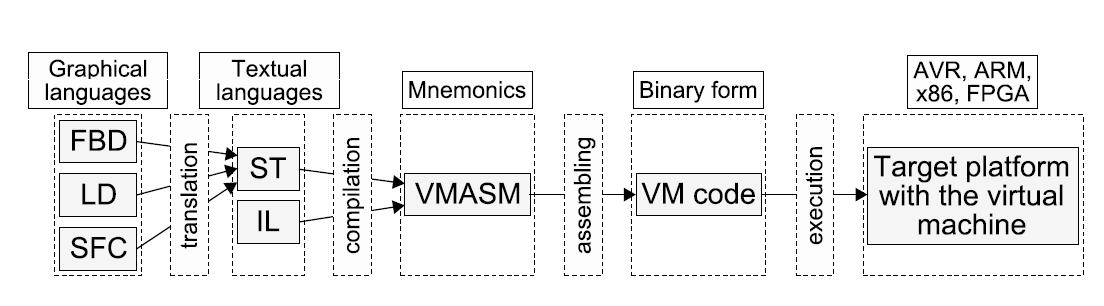
\includegraphics[width=15cm]{images/cpdevScheme.png}
   \caption{Schemat przetwarzania kodu użytkownika w środowisku CPDev\cite{cpdevOperations}}
   \label{Fig:cpdevScheme}
\end{figure}

\clearpage

\section{Drzewa składniowe na podstawie gramatyki bezkontekstowej}
\subsection{Wprowadzenie do gramatyk bezkontekstowych}
Gramatyka bezkontekstowa (CFG, Context-Free Grammar) to matematyczny model służący do opisu struktury formalnych języków, takich jak języki programowania. Składa się z: skończonego zbioru symboli nieterminalnych (zmiennych), zbioru symboli terminalnych (symboli końcowych, np. słów kluczowych, operatorów), zestawu produkcyjnych reguł, w których każdy symbol nieteminalny może być zastąpiony ciągiem terminali i/lub nieterminali, specjalnego symbolu startowego. Najważniejszą ich cechą jest to, że zachowują swoje znaczenie niezależnie od kontekstu czyli otoczenia w którym znajduje się symbol. Gramatyki bezkontekstowe są wystarczająco wyraźne, by opisać większość języków programowania, ale jednocześnie na tyle proste, by dawać się wydajnie parsować algorytmicznie.\cite{contextFreeGrammar}

\subsection{Wyprowadzenia i formy zdaniowe}
Proces generowania ciągu terminali rozpoczyna się od symbolu startowego i polega na wielokrotnym zastępowaniu nieterminali zgodnie z regułami gramatyki rozwijając kolejno każdy symbol nieterminalny\cite{contextFreeGrammar}. Taki proces to wyprowadzanie, często opisywany za pomocą kroków typu lewostronnego lub prawostronnego. W każdym etapie generowania teminali powstają tzw. formy zdaniowe, czyli częściowo przetworzone ciągi symboli.

\subsection{Drzewa składniowe}
Drzewo składniowe to uporządkowana struktura w postaci drzewa, która wizualnie i strukturalnie odwzorowuje sposób, w jaki ciąg symboli terminalnych (np. kod programu) został wygenerowany przez gramatykę. Korzeń drzewa to symbol startowy, a każdy węzeł wewnętrzny reprezentuje symbol nieterminalny, który został rozwinięty na swoje dzieci (symboli terminalnych lub innych nieterminali). Z kolei liście drzewa odpowiadają symbolom terminalnym, które są końcowymi elementami wygenerowanego ciągu.

Drzewo składniowe powstaje podczas parsowania: każda reguła produkcji zamienia symbol nieterminalny na jego dzieci w drzewie. Korzystając z kolejności liści od lewej lub prawej, odczytujemy oryginalny ciąg słów, czyli kod źródłowy. Poniżej na rysunku \ref{Fig:simpleGrammarTree} przedstawiono przykład drzewa składniowego dla prostego wyrażenia arytmetycznego \textit{7 + 2 * 3} z zastosowaniem zasad znanych z matematyki, gdzie mnożenie ma wyższy priorytet niż dodawanie.

\begin{figure}[ht]
   \centering
   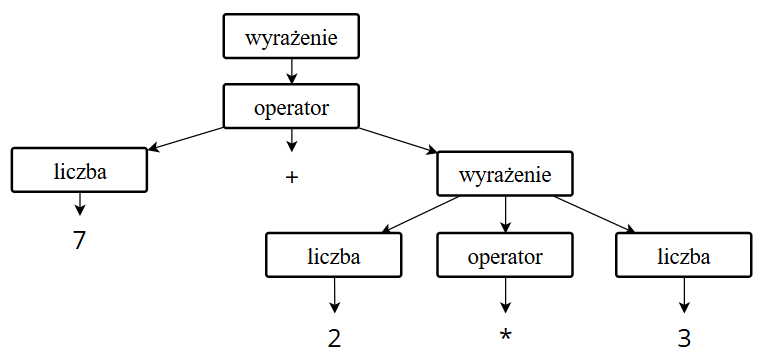
\includegraphics[width=15cm]{images/grammarTreeSimple.png}
   \caption{Drzewo składniowe dla prostego wyrażenia arytemtycznego \textit{7 + 2 * 3}}
   \label{Fig:simpleGrammarTree}
\end{figure}


Drzewa składniowe mogą służyć jako:
\begin{itemize}[label=\textbullet, leftmargin=1.25cm]
   \item reprezentacja struktury kodu źródłowego, na przejrzystym drzewie,
   \item podstawa do analiz semantycznych, takich jak sprawdzanie typów czy wykrywanie błędów,
   \item model do generacji kodu pośredniego lub docelowego wykorzystywany kompilatorach i interpreterach.
\end{itemize}

\subsection{Zastosowanie parserów w IDE i narzędziach}
W zintegrowanych środowiskach programistycznych drzewa składniowe umożliwiają kolorowanie składni, dynamiczne podpowiedzi, sprawdzanie błędów składniowych, a także refaktoryzację kodu. Dla CPDev-a z uwagi na to, że korzysta on z translatora kodu źródłowego, drzewo składniowe kodu języka ST jest niezbędne do poprawnej analizy i interpretacji kodu. Automatyczna generacja drzewa składniowego na podstawie pliku gramatyki pozwoliłaby na ujednolicenie procesu tworzenia parsera, co jest niezwykle istotne w kontekście rozwoju środowiska CPDev. Dzięki temu możliwe byłoby łatwiejsze wprowadzanie zmian w gramatyce języka ST oraz szybsze dostosowywanie parsera do nowych wymagań.
\clearpage

\section{Przegląd narzędzi do automatycznego generowania drzew składni}
\subsection{Bison}
\lstinputlisting[inputencoding=utf8/cp1250, language={C++}, caption={\protect\input{captions/drawMoveUp.txt}\protect\relax}, label={Lst:drawMoveUp}]{codes/drawMoveUp.cpp}
\subsection{Irony.Net}
\subsection{ANTLRv4}
\subsection{Porównanie}
\clearpage
\section{Utworzenie parsera języka ST przy pomocy ANTLRv4}
\subsection{Przygotowanie środowiska i utworzenie struktury projektu}
\subsection{Gramatyka - lexer}
\subsection{Gramatyka - parser}
\subsection{Ocena przygotowanego oprogamowania}
\clearpage

\section{Zakończenie}

Niniejsza praca miała na celu zaproponowanie rozwiązania sterowania telewizorem z poziomu smartfona dzięki aplikacji mobilnej i urządzeniu pośredniczącym opartemu o mikrokontroler z niezbędnymi modułami. Omówiono w niej technologie i~koncepty, z których korzystano podczas procesu projektowania tego systemu. Opisane zostały też najważniejsze elementy fizycznej części projektu, oprogramowanie mikrokontrolera, zbudowana aplikacja mobilna oraz ich współpraca w cely sterowania telewizorem.

Utworzony prototyp systemu zapewnił możliwość programowania przycisków pilota w aplikacji mobilnej w oparciu o szesnastkowe kody sygnałów podczerwonych. Kody te można uzyskać przeglądając sieć i strony producentów urządzeń multimedialnych oraz dzięki wbudowanemu w urządzenie pośredniczące czytnikowi kodów IR, który po odebraniu takiego kodu przez podczerwień, wyświetla go na ekranie OLED. Przy pomocy serwera BLE zastosowanego na urządzeniu wysyłającym sygnały podczerwone zapewniono także dostęp do systemu dla wielu użytkowników jednocześnie. Utworzona aplikacja mobilna jest prosta w użytkowaniu i intuicyjna nawet dla użytkowników nieobytych z technologią obecną w dzisiejszych smartfonach, a duże i wyraziste elementy pozwalają się dostrzec nawet z większych odległości.

Zaprojektowany prototypowy system aplikacji mobilnej i urządzenia pośredniczącego opartego o mikrokontroler jest już w pełni funkcjonalny i może nawet zostać przekształcony do produktu komercyjnego. Aby zwiększyć jednak atrakcyjność tego rozwiązania na rynku, można wskazać kilka usprawnień jak na przykład:
\begin{itemize}[label=-,labelsep=0.4cm,leftmargin=0.65cm]
   \item zamknięcie urządzenia pośredniczącego w wygodnej prostokątnej obudowie z odpowiednim rozłożeniem modułów,
   \item wprowadznie automatyzacji programowania kodów IR i wczytywania ich z plików JSON, udostępnianych też na stronie internetowej firmy,
   \item dodanie obsługi inteligentnych gestów użytkownika w aplikacji dla konkretnych typów urządzeń,
   \item wprowadzenie kreatora ekranów przycisków pilota w aplikacji dla maksymalnej uniwersalności rozwiązania,
   \item wprowadzenie systemu logowania, aby przechowywać zestawy przycisków na serwerze, dzięki czemu będą one dostępne dla wielu urządzeń tego użytkownika
   
\end{itemize}

Autor za własny wkład pracy uważa: 
\begin{itemize}[label=-,labelsep=0.4cm,leftmargin=0.65cm]
   \item przegląd i dobór technologii do utworzonego rozwiązania,
   \item zaprojektowanie urządzenia pośredniczącego opartego o mikrokontroler wysyłającego i odbierającego sygnały IR,
   \item zaprojektowanie interfejsu użytkownika aplikacji mobilnej,
   \item zaprojektowanie komunikacji aplikacji mobilnej pilota uniwersalnego z mikrokontrolerem w oparciu o~technologię BLE,
   \item utworzenie odpowiedniego oprogramowania sterującego dla mikrokontrolera,
   \item zbudowanie i oprogramowanie aplikacji mobilnej,
   \item opis oprogramowania i przedstawienie elementów utworzonego systemu.
   
\end{itemize}

\clearpage
\addcontentsline{toc}{section}{Literatura}
\bibliography{biblgr}
\bibliographystyle{plain}

\clearpage

\makesummary

\end{document}
